\documentclass{article}

\usepackage{graphicx}
\usepackage{amsmath}
\usepackage{amsthm}
\usepackage{amssymb}
\usepackage{fancyhdr}
\usepackage{hyperref}
\usepackage[dvipsnames]{xcolor}
\usepackage{enumitem}
\usepackage{xcolor}
\usepackage{minted}
%%%%% NEW MATH DEFINITIONS %%%%%

\usepackage{amsmath,amsfonts,bm,bbm}

\def\ind{{\mathbbm{1}}}

% Mark sections of captions for referring to divisions of figures
\newcommand{\figleft}{{\em (Left)}}
\newcommand{\figcenter}{{\em (Center)}}
\newcommand{\figright}{{\em (Right)}}
\newcommand{\figtop}{{\em (Top)}}
\newcommand{\figbottom}{{\em (Bottom)}}
\newcommand{\captiona}{{\em (a)}}
\newcommand{\captionb}{{\em (b)}}
\newcommand{\captionc}{{\em (c)}}
\newcommand{\captiond}{{\em (d)}}
\newcommand{\figleftt}{{\em Left}}
\newcommand{\figcentert}{{\em Center}}
\newcommand{\figrightt}{{\em Right}}
\newcommand{\figtopt}{{\em Top}}
\newcommand{\figbottomt}{{\em Bottom}}
\newcommand{\captionat}{{\em a}}
\newcommand{\captionbt}{{\em b}}
\newcommand{\captionct}{{\em c}}
\newcommand{\captiondt}{{\em d}}

% Highlight a newly defined term
\newcommand{\newterm}[1]{{\bf #1}}


% Figure reference, lower-case.
\def\figref#1{figure~\ref{#1}}
% Figure reference, capital. For start of sentence
\def\Figref#1{Figure~\ref{#1}}
\def\twofigref#1#2{figures \ref{#1} and \ref{#2}}
\def\quadfigref#1#2#3#4{figures \ref{#1}, \ref{#2}, \ref{#3} and \ref{#4}}
% Section reference, lower-case.
\def\secref#1{section~\ref{#1}}
% Section reference, capital.
\def\Secref#1{Section~\ref{#1}}
% Reference to two sections.
\def\twosecrefs#1#2{sections \ref{#1} and \ref{#2}}
% Reference to three sections.
\def\secrefs#1#2#3{sections \ref{#1}, \ref{#2} and \ref{#3}}

\def\chapref#1{chapter~\ref{#1}}
% Reference to an equation, upper case.
\def\Chapref#1{Chapter~\ref{#1}}
% Reference to a range of chapters
\def\rangechapref#1#2{chapters\ref{#1}--\ref{#2}}
% Reference to an algorithm, lower-case.
\def\algref#1{algorithm~\ref{#1}}
% Reference to an algorithm, upper case.
\def\Algref#1{Algorithm~\ref{#1}}
\def\twoalgref#1#2{algorithms \ref{#1} and \ref{#2}}
\def\Twoalgref#1#2{Algorithms \ref{#1} and \ref{#2}}
% Reference to a part, lower case
\def\partref#1{part~\ref{#1}}
% Reference to a part, upper case
\def\Partref#1{Part~\ref{#1}}
\def\twopartref#1#2{parts \ref{#1} and \ref{#2}}

\def\ceil#1{\lceil #1 \rceil}
\def\floor#1{\lfloor #1 \rfloor}
\def\1{\bm{1}}
\newcommand{\train}{\mathcal{D}}
\newcommand{\valid}{\mathcal{D_{\mathrm{valid}}}}
\newcommand{\test}{\mathcal{D_{\mathrm{test}}}}

\def\eps{{\epsilon}}


% Random variables
\def\reta{{\textnormal{$\eta$}}}
\def\ra{{\textnormal{a}}}
\def\rb{{\textnormal{b}}}
\def\rc{{\textnormal{c}}}
\def\rd{{\textnormal{d}}}
\def\re{{\textnormal{e}}}
\def\rf{{\textnormal{f}}}
\def\rg{{\textnormal{g}}}
\def\rh{{\textnormal{h}}}
\def\ri{{\textnormal{i}}}
\def\rj{{\textnormal{j}}}
\def\rk{{\textnormal{k}}}
\def\rl{{\textnormal{l}}}
% rm is already a command, just don't name any random variables m
\def\rn{{\textnormal{n}}}
\def\ro{{\textnormal{o}}}
\def\rp{{\textnormal{p}}}
\def\rq{{\textnormal{q}}}
\def\rr{{\textnormal{r}}}
\def\rs{{\textnormal{s}}}
\def\rt{{\textnormal{t}}}
\def\ru{{\textnormal{u}}}
\def\rv{{\textnormal{v}}}
\def\rw{{\textnormal{w}}}
\def\rx{{\textnormal{x}}}
\def\ry{{\textnormal{y}}}
\def\rz{{\textnormal{z}}}

% Random vectors
\def\rvepsilon{{\mathbf{\epsilon}}}
\def\rvtheta{{\mathbf{\theta}}}
\def\rva{{\mathbf{a}}}
\def\rvb{{\mathbf{b}}}
\def\rvc{{\mathbf{c}}}
\def\rvd{{\mathbf{d}}}
\def\rve{{\mathbf{e}}}
\def\rvf{{\mathbf{f}}}
\def\rvg{{\mathbf{g}}}
\def\rvh{{\mathbf{h}}}
\def\rvu{{\mathbf{i}}}
\def\rvj{{\mathbf{j}}}
\def\rvk{{\mathbf{k}}}
\def\rvl{{\mathbf{l}}}
\def\rvm{{\mathbf{m}}}
\def\rvn{{\mathbf{n}}}
\def\rvo{{\mathbf{o}}}
\def\rvp{{\mathbf{p}}}
\def\rvq{{\mathbf{q}}}
\def\rvr{{\mathbf{r}}}
\def\rvs{{\mathbf{s}}}
\def\rvt{{\mathbf{t}}}
\def\rvu{{\mathbf{u}}}
\def\rvv{{\mathbf{v}}}
\def\rvw{{\mathbf{w}}}
\def\rvx{{\mathbf{x}}}
\def\rvy{{\mathbf{y}}}
\def\rvz{{\mathbf{z}}}

% Elements of random vectors
\def\erva{{\textnormal{a}}}
\def\ervb{{\textnormal{b}}}
\def\ervc{{\textnormal{c}}}
\def\ervd{{\textnormal{d}}}
\def\erve{{\textnormal{e}}}
\def\ervf{{\textnormal{f}}}
\def\ervg{{\textnormal{g}}}
\def\ervh{{\textnormal{h}}}
\def\ervi{{\textnormal{i}}}
\def\ervj{{\textnormal{j}}}
\def\ervk{{\textnormal{k}}}
\def\ervl{{\textnormal{l}}}
\def\ervm{{\textnormal{m}}}
\def\ervn{{\textnormal{n}}}
\def\ervo{{\textnormal{o}}}
\def\ervp{{\textnormal{p}}}
\def\ervq{{\textnormal{q}}}
\def\ervr{{\textnormal{r}}}
\def\ervs{{\textnormal{s}}}
\def\ervt{{\textnormal{t}}}
\def\ervu{{\textnormal{u}}}
\def\ervv{{\textnormal{v}}}
\def\ervw{{\textnormal{w}}}
\def\ervx{{\textnormal{x}}}
\def\ervy{{\textnormal{y}}}
\def\ervz{{\textnormal{z}}}

% Random matrices
\def\rmA{{\mathbf{A}}}
\def\rmB{{\mathbf{B}}}
\def\rmC{{\mathbf{C}}}
\def\rmD{{\mathbf{D}}}
\def\rmE{{\mathbf{E}}}
\def\rmF{{\mathbf{F}}}
\def\rmG{{\mathbf{G}}}
\def\rmH{{\mathbf{H}}}
\def\rmI{{\mathbf{I}}}
\def\rmJ{{\mathbf{J}}}
\def\rmK{{\mathbf{K}}}
\def\rmL{{\mathbf{L}}}
\def\rmM{{\mathbf{M}}}
\def\rmN{{\mathbf{N}}}
\def\rmO{{\mathbf{O}}}
\def\rmP{{\mathbf{P}}}
\def\rmQ{{\mathbf{Q}}}
\def\rmR{{\mathbf{R}}}
\def\rmS{{\mathbf{S}}}
\def\rmT{{\mathbf{T}}}
\def\rmU{{\mathbf{U}}}
\def\rmV{{\mathbf{V}}}
\def\rmW{{\mathbf{W}}}
\def\rmX{{\mathbf{X}}}
\def\rmY{{\mathbf{Y}}}
\def\rmZ{{\mathbf{Z}}}
\def\rmtheta{{\mathbf{\Theta}}}
% Elements of random matrices
\def\ermA{{\textnormal{A}}}
\def\ermB{{\textnormal{B}}}
\def\ermC{{\textnormal{C}}}
\def\ermD{{\textnormal{D}}}
\def\ermE{{\textnormal{E}}}
\def\ermF{{\textnormal{F}}}
\def\ermG{{\textnormal{G}}}
\def\ermH{{\textnormal{H}}}
\def\ermI{{\textnormal{I}}}
\def\ermJ{{\textnormal{J}}}
\def\ermK{{\textnormal{K}}}
\def\ermL{{\textnormal{L}}}
\def\ermM{{\textnormal{M}}}
\def\ermN{{\textnormal{N}}}
\def\ermO{{\textnormal{O}}}
\def\ermP{{\textnormal{P}}}
\def\ermQ{{\textnormal{Q}}}
\def\ermR{{\textnormal{R}}}
\def\ermS{{\textnormal{S}}}
\def\ermT{{\textnormal{T}}}
\def\ermU{{\textnormal{U}}}
\def\ermV{{\textnormal{V}}}
\def\ermW{{\textnormal{W}}}
\def\ermX{{\textnormal{X}}}
\def\ermY{{\textnormal{Y}}}
\def\ermZ{{\textnormal{Z}}}

% Vectors
\def\vzero{{\bm{0}}}
\def\vone{{\bm{1}}}
\def\vmu{{\bm{\mu}}}
\def\vtheta{{\bm{\theta}}}
\def\va{{\bm{a}}}
\def\vb{{\bm{b}}}
\def\vc{{\bm{c}}}
\def\vd{{\bm{d}}}
\def\ve{{\bm{e}}}
\def\vf{{\bm{f}}}
\def\vg{{\bm{g}}}
\def\vh{{\bm{h}}}
\def\vi{{\bm{i}}}
\def\vj{{\bm{j}}}
\def\vk{{\bm{k}}}
\def\vl{{\bm{l}}}
\def\vm{{\bm{m}}}
\def\vn{{\bm{n}}}
\def\vo{{\bm{o}}}
\def\vp{{\bm{p}}}
\def\vq{{\bm{q}}}
\def\vr{{\bm{r}}}
\def\vs{{\bm{s}}}
\def\vt{{\bm{t}}}
\def\vu{{\bm{u}}}
\def\vv{{\bm{v}}}
\def\vw{{\bm{w}}}
\def\vx{{\bm{x}}}
\def\vy{{\bm{y}}}
\def\vz{{\bm{z}}}

% Elements of vectors
\def\evalpha{{\alpha}}
\def\evbeta{{\beta}}
\def\evepsilon{{\epsilon}}
\def\evlambda{{\lambda}}
\def\evomega{{\omega}}
\def\evmu{{\mu}}
\def\evpsi{{\psi}}
\def\evsigma{{\sigma}}
\def\evtheta{{\theta}}
\def\eva{{a}}
\def\evb{{b}}
\def\evc{{c}}
\def\evd{{d}}
\def\eve{{e}}
\def\evf{{f}}
\def\evg{{g}}
\def\evh{{h}}
\def\evi{{i}}
\def\evj{{j}}
\def\evk{{k}}
\def\evl{{l}}
\def\evm{{m}}
\def\evn{{n}}
\def\evo{{o}}
\def\evp{{p}}
\def\evq{{q}}
\def\evr{{r}}
\def\evs{{s}}
\def\evt{{t}}
\def\evu{{u}}
\def\evv{{v}}
\def\evw{{w}}
\def\evx{{x}}
\def\evy{{y}}
\def\evz{{z}}

% Matrix
\def\mA{{\bm{A}}}
\def\mB{{\bm{B}}}
\def\mC{{\bm{C}}}
\def\mD{{\bm{D}}}
\def\mE{{\bm{E}}}
\def\mF{{\bm{F}}}
\def\mG{{\bm{G}}}
\def\mH{{\bm{H}}}
\def\mI{{\bm{I}}}
\def\mJ{{\bm{J}}}
\def\mK{{\bm{K}}}
\def\mL{{\bm{L}}}
\def\mM{{\bm{M}}}
\def\mN{{\bm{N}}}
\def\mO{{\bm{O}}}
\def\mP{{\bm{P}}}
\def\mQ{{\bm{Q}}}
\def\mR{{\bm{R}}}
\def\mS{{\bm{S}}}
\def\mT{{\bm{T}}}
\def\mU{{\bm{U}}}
\def\mV{{\bm{V}}}
\def\mW{{\bm{W}}}
\def\mX{{\bm{X}}}
\def\mY{{\bm{Y}}}
\def\mZ{{\bm{Z}}}
\def\mBeta{{\bm{\beta}}}
\def\mPhi{{\bm{\Phi}}}
\def\mLambda{{\bm{\Lambda}}}
\def\mSigma{{\bm{\Sigma}}}

% Tensor
\DeclareMathAlphabet{\mathsfit}{\encodingdefault}{\sfdefault}{m}{sl}
\SetMathAlphabet{\mathsfit}{bold}{\encodingdefault}{\sfdefault}{bx}{n}
\newcommand{\tens}[1]{\bm{\mathsfit{#1}}}
\def\tA{{\tens{A}}}
\def\tB{{\tens{B}}}
\def\tC{{\tens{C}}}
\def\tD{{\tens{D}}}
\def\tE{{\tens{E}}}
\def\tF{{\tens{F}}}
\def\tG{{\tens{G}}}
\def\tH{{\tens{H}}}
\def\tI{{\tens{I}}}
\def\tJ{{\tens{J}}}
\def\tK{{\tens{K}}}
\def\tL{{\tens{L}}}
\def\tM{{\tens{M}}}
\def\tN{{\tens{N}}}
\def\tO{{\tens{O}}}
\def\tP{{\tens{P}}}
\def\tQ{{\tens{Q}}}
\def\tR{{\tens{R}}}
\def\tS{{\tens{S}}}
\def\tT{{\tens{T}}}
\def\tU{{\tens{U}}}
\def\tV{{\tens{V}}}
\def\tW{{\tens{W}}}
\def\tX{{\tens{X}}}
\def\tY{{\tens{Y}}}
\def\tZ{{\tens{Z}}}


% Graph
\def\gA{{\mathcal{A}}}
\def\gB{{\mathcal{B}}}
\def\gC{{\mathcal{C}}}
\def\gD{{\mathcal{D}}}
\def\gE{{\mathcal{E}}}
\def\gF{{\mathcal{F}}}
\def\gG{{\mathcal{G}}}
\def\gH{{\mathcal{H}}}
\def\gI{{\mathcal{I}}}
\def\gJ{{\mathcal{J}}}
\def\gK{{\mathcal{K}}}
\def\gL{{\mathcal{L}}}
\def\gM{{\mathcal{M}}}
\def\gN{{\mathcal{N}}}
\def\gO{{\mathcal{O}}}
\def\gP{{\mathcal{P}}}
\def\gQ{{\mathcal{Q}}}
\def\gR{{\mathcal{R}}}
\def\gS{{\mathcal{S}}}
\def\gT{{\mathcal{T}}}
\def\gU{{\mathcal{U}}}
\def\gV{{\mathcal{V}}}
\def\gW{{\mathcal{W}}}
\def\gX{{\mathcal{X}}}
\def\gY{{\mathcal{Y}}}
\def\gZ{{\mathcal{Z}}}

% Sets
\def\sA{{\mathbb{A}}}
\def\sB{{\mathbb{B}}}
\def\sC{{\mathbb{C}}}
\def\sD{{\mathbb{D}}}
% Don't use a set called E, because this would be the same as our symbol
% for expectation.
\def\sF{{\mathbb{F}}}
\def\sG{{\mathbb{G}}}
\def\sH{{\mathbb{H}}}
\def\sI{{\mathbb{I}}}
\def\sJ{{\mathbb{J}}}
\def\sK{{\mathbb{K}}}
\def\sL{{\mathbb{L}}}
\def\sM{{\mathbb{M}}}
\def\sN{{\mathbb{N}}}
\def\sO{{\mathbb{O}}}
\def\sP{{\mathbb{P}}}
\def\sQ{{\mathbb{Q}}}
\def\sR{{\mathbb{R}}}
\def\sS{{\mathbb{S}}}
\def\sT{{\mathbb{T}}}
\def\sU{{\mathbb{U}}}
\def\sV{{\mathbb{V}}}
\def\sW{{\mathbb{W}}}
\def\sX{{\mathbb{X}}}
\def\sY{{\mathbb{Y}}}
\def\sZ{{\mathbb{Z}}}

% Entries of a matrix
\def\emLambda{{\Lambda}}
\def\emA{{A}}
\def\emB{{B}}
\def\emC{{C}}
\def\emD{{D}}
\def\emE{{E}}
\def\emF{{F}}
\def\emG{{G}}
\def\emH{{H}}
\def\emI{{I}}
\def\emJ{{J}}
\def\emK{{K}}
\def\emL{{L}}
\def\emM{{M}}
\def\emN{{N}}
\def\emO{{O}}
\def\emP{{P}}
\def\emQ{{Q}}
\def\emR{{R}}
\def\emS{{S}}
\def\emT{{T}}
\def\emU{{U}}
\def\emV{{V}}
\def\emW{{W}}
\def\emX{{X}}
\def\emY{{Y}}
\def\emZ{{Z}}
\def\emSigma{{\Sigma}}

% entries of a tensor
% Same font as tensor, without \bm wrapper
\newcommand{\etens}[1]{\mathsfit{#1}}
\def\etLambda{{\etens{\Lambda}}}
\def\etA{{\etens{A}}}
\def\etB{{\etens{B}}}
\def\etC{{\etens{C}}}
\def\etD{{\etens{D}}}
\def\etE{{\etens{E}}}
\def\etF{{\etens{F}}}
\def\etG{{\etens{G}}}
\def\etH{{\etens{H}}}
\def\etI{{\etens{I}}}
\def\etJ{{\etens{J}}}
\def\etK{{\etens{K}}}
\def\etL{{\etens{L}}}
\def\etM{{\etens{M}}}
\def\etN{{\etens{N}}}
\def\etO{{\etens{O}}}
\def\etP{{\etens{P}}}
\def\etQ{{\etens{Q}}}
\def\etR{{\etens{R}}}
\def\etS{{\etens{S}}}
\def\etT{{\etens{T}}}
\def\etU{{\etens{U}}}
\def\etV{{\etens{V}}}
\def\etW{{\etens{W}}}
\def\etX{{\etens{X}}}
\def\etY{{\etens{Y}}}
\def\etZ{{\etens{Z}}}


\DeclareMathOperator{\E}{\mathbb{E}}
\newcommand{\Ls}{\mathcal{L}}
\newcommand{\R}{\mathbb{R}}
\newcommand{\emp}{\tilde{p}}
\newcommand{\lr}{\alpha}
\newcommand{\reg}{\lambda}
\newcommand{\sigmoid}{\sigma}
\newcommand{\softplus}{\zeta}
\newcommand{\KL}{D_{\mathrm{KL}}}
\newcommand{\Var}{\mathrm{Var}}
\newcommand{\standarderror}{\mathrm{SE}}
\newcommand{\Cov}{\mathrm{Cov}}
\DeclareMathOperator*{\argmax}{arg\,max}
\DeclareMathOperator*{\argmin}{arg\,min}

\DeclareMathOperator{\sign}{sign}
\DeclareMathOperator{\Tr}{Tr}
\let\ab\allowbreak

\newcommand{\vbar}[1]{\bigg\rvert_{#1}}
\newcommand\at[2]{\left.#1\right|_{#2}}
\newcommand{\bs}[1]{\boldsymbol{#1}}

\newcommand{\sigx}[1]{\sigma_{x,#1}}
\newcommand{\sigb}[1]{\sigma_{\beta,#1}}

\newcommand{\dd}{\mathrm{d}} %for integration
\usepackage{amsmath,amssymb,amsfonts,amsthm}

\newcommand{\wipcom}[1]{\textcolor{red}{WIP: #1}}
\newcommand{\sol}[1]{\textcolor{gray}{Solution: #1}}
\newcommand{\nyuparagrah}[1]{\textcolor{nyupurple}{\large #1}}
\newcommand{\code}[1]{\texttt{#1}}

\pagestyle{empty} \addtolength{\textwidth}{1.0in}
\addtolength{\textheight}{0.5in} \addtolength{\oddsidemargin}{-0.5in}
\addtolength{\evensidemargin}{0.5in}
\newcommand{\ruleskip}{\bigskip\hrule\bigskip}
\newcommand{\nodify}[1]{{\sc #1}} \newcommand{\points}[1]{{\textbf{[#1
points]}}}

\newcommand{\bitem}{\begin{list}{$\bullet$}%
{\setlength{\itemsep}{0pt}\setlength{\topsep}{0pt}%
\setlength{\rightmargin}{0pt}}} \newcommand{\eitem}{\end{list}}

\definecolor{nyupurple}{RGB}{134, 0, 179}
\setlength{\parindent}{0pt} \setlength{\parskip}{0.5ex}

\DeclareUnicodeCharacter{2212}{-}

\theoremstyle{plain}
\newtheorem*{thm*}{\protect\theoremname}
\theoremstyle{definition}
\newtheorem*{defn*}{\protect\definitionname}

\begin{document}
\newcounter{saveenum}

\pagestyle{myheadings} \markboth{}{\color{nyupurple} DS-GA-1003 - Spring 2023}

\begin{center}
{\Large
Homework 3: SVMs \& Kernel Methods
} 
\end{center}

{
{ \color{nyupurple} \textbf{Due:} Wednesday, March 1, 2023 at 11:59PM EST} 
} 

\textbf{Instructions: }Your answers to the questions below, including plots and mathematical
 work, should be submitted as a single PDF file.  It's preferred that you write your answers using software that typesets mathematics (e.g.LaTeX, LyX, or MathJax via iPython), though if you need to you may scan handwritten work.  You may find the \href{https://github.com/gpoore/minted}{minted} package convenient for including source code in your LaTeX document.  If you are using LyX, then the \href{https://en.wikibooks.org/wiki/LaTeX/Source_Code_Listings}{listings} package tends to work better. \\
\ruleskip

% \wipcom{Clarify the support codes + location of data files}
In this problem set we will get up to speed with SVMs and Kernels. Long at first glance, the problem set includes a lot of helpers. You will find a review of kernalization. One section will include a revision of ridge regression which you should start to be familiar with. For the second and third problem some codes are provided to save you some time. Finally, some reminders on positive (semi)definite matrices are included in the Appendix.

\section{\large Support Vector Machines: SVMs with Pegasos}

In this first problem we will use Support Vector Machines to predict whether the sentiment of a movie review was \emph{positive} or \emph{negative}. We will represent each review by a vector $\bs x \in \sR^d$ where $d$ is the size of the word dictionary and $x_i$ is equal to the number of occurrence of the $i$-th word in the review $\bs x$. The corresponding label is either $y=1$ for a positive review or $y=-1$ for a negative review.
In class we have seen how to transform the SVM training objective into a quadratic program using the dual formulation. Here we will use a gradient descent algorithm instead.

\nyuparagrah{\bf Subgradients} 

Recall that a vector $g\in\mathbb{R}^{d}$ is a \emph{subgradient} of
$f:\mathbb{R}^{d}\to\mathbb{R}$ at $\bs x$ if for all $\bs z$, 
\[
f(\bs z)\ge f(\bs x)+g^{T}(\bs z- \bs x).
\]
There may be $0$, $1$, or infinitely many
subgradients at any point. The \emph{subdifferential} of $f$ at
a point $\bs x$, denoted $\partial f(\bs x)$, is the set of all subgradients
of $f$ at $\bs x$. 
% Just as there is a calculus for gradients, there is a calculus for
% subgradients
% \footnote{
  A good reference for subgradients are the \href{https://stanford.edu/class/ee364b/lectures/subgradients_notes.pdf}{course notes on Subgradients by Boyd et al}.
  % }.
%For our purposes, we can usually get by using the definition of subgradient
%directly. However, 
% In the first problem 
Below we derive a property
that will make our life easier for finding a subgradient of the hinge
loss.

\begin{enumerate}
  \setcounter{enumi}{\value{saveenum}}
\item Suppose $f_{1},\ldots,f_{m}:\mathbb{R}^{d}\to\mathbb{R}$
are convex functions, and 
% \[
$f(\bs x)=\max_{i=1,\ldots,,m}f_{i}(\bs x)$.
% \]
Let $k$ be any index for which $f_{k}(\bs x)=f(\bs x)$, and choose $g\in\partial f_{k}((\bs x)$ (a convex function on $\mathbb{R}^{d}$ has
a non-empty subdifferential at all points). Show that $g\in\partial f(\bs x)$.

\begin{itemize}
    \color{blue}
    \item we can show this directly 
    \item  as $f_k(x)=f(x)$ and $g\in \partial f(x)$ it must be the case $\forall z\in \mathbb{R}^d$ $f_{k}(z)\geq f_k(x)+g^{t}(z-x)$
    \item this allows us to write $ f_k(x)+g^{t}(z-x)=max(f_1(x)...f_n(x))+g^{t}(z-x)\geq f_i(x)+g^{t}(z-x) \forall i \in [1..m]$ and then by the definition of $f(x)$ we can say $\forall z\in \mathbb{R}^d  f(z)=max(f_1(z)...f_m(z))\geq f_k(z)\geq f_k(x)+g^{t}(z-x)=max(f_1(x)...f_n(x))+g^{t}(z-x)=f(x)+g^{t}(z-x)$
    \item meaning $\forall z\in \mathbb{R}^d  f(z)\geq f(x)+g^{t}(z-x)\Rightarrow g\in \partial f(x)$
\end{itemize}



\item Give a subgradient of the hinge loss objective
% \[
$J(\bs w)=\max\left\{ 0,1-y \bs w^{T} \bs x\right\}$.
% \]
\begin{itemize}
    \color{blue}
    \item by the above problem we know that a sub gradient of a the max of a combination of convex functions at any given point x is given by a subgradient of the max of those functions. 
    \item it is clear that $f_1(w)=0$ is convex as it is constant. it is also clear that $f_2(w)=1-y_iw^tx$ is convex in w as it is linear in w . 
    \item thus the subgradient for $j(w)$ at the point of discontinuity that is when $y_{i}w^{t}x_i=1$, will be given a subgradient of either $f_1(w)=0$ or $f_2(2)=1-y_iw^tx_i$ as at that point $0=1-y_iw^wx_i$ and thus $f_1(w)f_2(w)$
    \item further we know that for differentiable convex functions there subgradient are there gradients. 
    \item so in other words any linear combination of the gradients of $0,1-y_iw^tx_i$ will be a subgradient of $j(w)$ when $y_iw^tx_i=1$ 
    \item so our overall hinge loss subgradient is  $ \partial J(w)$ = \left \{ \begin{array}{lll} 0 \quad \text{if } y_{i}w^{t}x_i >1 \\ -y_ix_i \quad \text{if } y_{i}w^{t}x_i<1\\ \theta(-y_ix_i) \quad \text{ else} \end{array} \\$ where $\theta\in[0,1]$
\end{itemize}
 
\item \textcolor{violet}{(Optional)} Suppose we have function $f:\mathbb{R}^n\rightarrow\mathbb{R}$ which is sub-differentiable everywhere, i.e. $\partial f\neq \emptyset$ for all $x\in\mathbb{R}^n$. Show that $f$ is convex. Note, in the general case, a function is convex if for all $x,y$ in the domain of $f$ and for all $\theta \in (0,1)$,
\begin{align*}
    \theta f(a)+(1-\theta)f(b) \geq f(\theta a+(1-\theta)(b))
\end{align*}

Hint: Suppose $f$ is not convex, then by definition, there exists a point in some interval: $x_0\in (a,b)$, such that $f(x_0)$ lies above the line connection $(a,f(a)), (b,f(b))$. Is this possible if the function s sub-differentiable everywhere? 
\begin{itemize}
\color{blue}
    \item Sup pose $f$ is not convex, then by definition, there exists a point in some interval: $x_0\in (a,b)$, such that $f(x_0)$ lies above the line connection $(a,f(a)), (b,f(b))$.
    \item we know f has a sub differentiable everywhere that is $\exists \sigma\in \mathbb{R}^{d}$ such that $\forall z\in \mathbb{R}^{d}$ $f(z)\geq f(x)+\sigma^t(z-x)$ including $x_0$
    \item we know that $x_0$ is is inbetween a and b. so then there must exist some combination $\theta a+ (1-\theta)b=x_0$ we know that 
    \item since $x_0$ has a subdiferntial it must be the case that $f(\theta a)\geq f(x_0)+\sigma(\theta a- x)\Rightarrow f(\theta a)-\sigma(\theta a-x_0)\geq f(x_0)$ and similary $f((1-\theta) b)\geq f(x_0)+\sigma((1-\theta) b- x_0)\Rightarrow f((1-\theta) b)-\sigma((1-\theta) b-x)\geq f(x_0)$
    \item then for any $\lambda \in [0,1]$ we can write $\lambda f(\theta a)-\lambda\sigma(\theta a-x_0)+(1-\lambda )f((1-\theta) b)-(1-\lambda )\sigma((1-\theta) b-x)\geq f(x_0)$
    \item this simpflies to $\lambda f(\theta a)+(1-\lambda)f((1-\theta)b)+\lambda \theta x_0 + (1-\lambda)(1-\theta)(x_0)+\lambda(\theta a)+(1-\lambda)(1-\theta b)=\lambda f(\theta a)+(1-\lambda)f((1-\theta)b)+x_0-x_0=\lambda f(\theta a)+(1-\lambda)f((1-\theta)b)\geq f(x_0)=f(\lambda (\theta a) +(1-\lambda) ((1-\theta) b)$
    \item meaning that $x_0$ is bellow the line conecting $a,b$ and thus the function is convex.
    
\end{itemize}

\setcounter{saveenum}{\value{enumi}}
\end{enumerate}

\nyuparagrah{\bf SVM with the Pegasos algorithm}

You will train a Support Vector Machine using the Pegasos algorithm
% To align with the notation used in the Pegasos paper
\footnote{Shalev-Shwartz et al. \href{http://ttic.uchicago.edu/~nati/Publications/PegasosMPB.pdf}{Pegasos: Primal Estimated sub-GrAdient SOlver for SVM}.}.
Recall the SVM objective using a linear predictor $f(\bs x) = \bs w ^T \bs x$ and the hinge loss:
\[
\min_{\bs w\in\mathbb{R}^{d}}\frac{\lambda}{2}\|\bs w\|^{2}+\frac{1}{n}\sum_{i=1}^{n}\max\left\{ 0,1-y_{i}\bs w^{T}\bs x_{i}\right\} ,
\]
where $n$ is the number of training examples and $d$ the size of the dictionary.
Note that, for simplicity, we are leaving off the 
% unregularized
bias
term $b$. Note also that we are using $\ell_2$ regularization with a parameter $\lambda$. Pegasos is stochastic subgradient descent using a step
size rule $\eta_{t}=1/\left(\lambda t\right)$ for iteration number $t$. The pseudocode is
given below:
\begin{center}
\begin{tabular}{l}
\hline 
Input: $\lambda>0$. Choose $w_{1}=0,t=0$\tabularnewline
While termination condition not met\tabularnewline
\ \ For $j=1,\ldots,n$ (assumes data is randomly permuted)\tabularnewline
\ \ \ \ $t=t+1$\tabularnewline
\ \ \ \ $\eta_{t}=1/\left(t\lambda\right)$;\tabularnewline
\ \ \ \ If $y_{j}w_{t}^{T}x_{j}<1$\tabularnewline
\ \ \ \ \ \ $w_{t+1}=(1-\eta_{t}\lambda)w_{t}+\eta_{t}y_{j}x_{j}$\tabularnewline
\ \ \ \ Else \tabularnewline
\ \ \ \ \ \ $w_{t+1}=(1-\eta_{t}\lambda)w_{t}$\tabularnewline
\hline 
\end{tabular}
\par\end{center}
\begin{enumerate}
  \setcounter{enumi}{\value{saveenum}}
\item Consider the SVM objective function for a single training point\footnote{Recall that if $i$ is selected uniformly from the set $\left\{ 1,\ldots,n\right\} $,
then this objective function has the same expected value
as the full SVM objective function.}: $J_{i}(\bs w)=\frac{\lambda}{2}\|\bs w\|^{2}+\max\left\{ 0,1-y_{i}\bs w^{T}\bs x_{i}\right\} $.
The function $J_{i}(\bs w)$ is not differentiable everywhere. Specify where the gradient of $J_{i}(w)$ is not defined. Give an expression for the gradient where it is defined.\\
\begin{itemize}
\color{blue}
    \item the objective function in this case is not differentiable when $y_iw^tx_i=1$
    \item this makes sense as at that point $0$ and $1-y_iw^tx_i$ have the same value, but there gradients are not equal so the function is not continuous or differentiable at that point. 
    \item when the gradient is defined we have  $ \nabla J_{i}(w)$ = \left \{ \begin{array}{lll} \lambda w-y_ix_i} \quad \text{if } y_{i}w^{t}x_i <1 \\ \lambda w \quad \text{if } y_{i}w^{t}x_i>1$\end{array}
\end{itemize}


\item Show that a subgradient of $J_{i}(w)$ is given by 
\begin{eqnarray*}
\bs g{\bs w} & = & \begin{cases}
\lambda \bs w-y_{i}\bs x_{i} & \mbox{for }y_{i}\bs w^{T}\bs x_{i}<1\\
\lambda \bs w & \mbox{for }y_{i}\bs w^{T}\bs x_{i}\ge1.
\end{cases}
\end{eqnarray*}
You may use the following facts without proof: 1) If $f_{1},\ldots,f_{n}:\mathbb{R}^{d}\to\mathbb{R}$
are convex functions and $f=f_{1}+\cdots+f_{n}$, then $\partial f(\bs x)=\partial f_{1}(\bs x)+\cdots+\partial f_{n}(\bs x)$.
2) For $\alpha\ge0$, $\partial\left(\alpha f\right)(x)=\alpha\partial f(x)$.
(Hint: Use the 
% rules provided and the calculation in the 
first part of this problem.)
\begin{itemize}
    \color{blue}
    \item first we want to show that $\frac{\lambda}{2}||w||^{2}_{2}$ is convex. we can see that the partial derivative of its gradient is $\lambda> 0$ for all values of w so thus it is convex
    \item next we want to show that $max(0,1-y_iw^tx_i)=max(f_1(w),f_2(w))$ is convex. $f''_1(w)=0\geq 0\forall w$ so $f_1$ is convex $f_{2}''(w)=0\geq 0$ so this it is also convex.  further we know that the max of two convex functions is also convex so thus  $max(0,1-y_iw^tx_i)$ is convex
    \item so now we can apply the first given fact to say $\partial j_i(w)=\partial \frac{1\lambda2}||w||^{2}_{2} + \partial max(0,1-y_iw^tx_i)=\lambda w+\partial max(0,1-y_iw^tx_i)$
    \item we showed earlier that our overall hinge loss subgradient is  $ \partial J(w)$ = \left \{ \begin{array}{lll} 0 \quad \text{if } y_{i}w^{t}x_i >1 \\ -y_ix_i \quad \text{if } y_{i}w^{t}x_i<1\\ \theta(-y_ix_i) \quad \text{ else} \end{array} \\$ where $\theta\in[0,1]$ 
    \item so the formulation given in the problem already holds bassed on that when $y_iw^tx_i\neq 1$
    \item furhter if we chose $\theta=1$ we can write using the second fact given in the problem $\partial max(0,1-y_iw^tx_i)=\theta(-y_ix_i)=-y_ix_i $
    \item thus we can see that a valid gradient for $j_i(w)$ is given by \begin{eqnarray*}
\bs g{\bs w} & = & \begin{cases}
\lambda \bs w-y_{i}\bs x_{i} & \mbox{for }y_{i}\bs w^{T}\bs x_{i}<1\\
\lambda \bs w & \mbox{for }y_{i}\bs w^{T}\bs x_{i}\ge1.
\end{cases}
\end{eqnarray*}
\item whcih is what we wanted to show
\end{itemize}


\setcounter{saveenum}{\value{enumi}}
\end{enumerate}

Convince yourself that if your step size rule is $\eta_{t}=1/\left(\lambda t\right)$,
then doing SGD with the subgradient direction from the previous question
is the same as given in the pseudocode. \\


\nyuparagrah{\bf Dataset and sparse representation} 

We will be using the \href{https://www.cs.cornell.edu/people/pabo/movie-review-data/}{Polarity Dataset v2.0},
constructed by Pang and Lee, provided in the \texttt{data\_reviews} folder. It has the full text from 2000 movies
reviews: 1000 reviews are classified as \emph{positive} and 1000 as
\emph{negative}. Our goal is to predict whether a review has positive
or negative sentiment from the text of the review. Each review is
stored in a separate file: the positive reviews are in a folder called
``pos'', and the negative reviews are in ``neg''. We have provided
some code in \texttt{utils\_svm\_reviews.py} to assist with reading these files.
% You can use the code, or write your own version. 
The code removes
some special symbols from the reviews and shuffles the data.
% \wipcom{Later you can check if this
% helps or hurts your results.}
Load all the data to have an idea of what it looks like.

A usual method to represent text documents in machine learning
is with \emph{bag-of-words}. As hinted above, here every possible word in the dictionnary
is a feature, and the value of a word feature for a given text is the number of times that word appears in the text. As most words will not
appear in any particular document, many of these counts will be zero.
Rather than storing many zeros, we use a \emph{sparse representation},
in which only the nonzero counts are tracked. The counts are
stored in a key/value data structure, such as a dictionary in Python. For
example, ``Harry Potter and Harry Potter II'' would be represented
as the following Python dict: \code{x=\{'Harry':2, 'Potter':2, 'and':1, 'II':1\}}.


\begin{enumerate}
  \setcounter{enumi}{\value{saveenum}}
\item Write a function that converts an example (a list of words) into
a sparse bag-of-words representation. You may find Python's Counter\footnote{\url{https://docs.python.org/2/library/collections.html}}
class to be useful here. Note that a Counter is itself a dictionary.
\begin{itemize}
    \color{blue}
      \inputminted[firstline=14, lastline=19, breaklines=True]{python}{hw_3.py}
\end{itemize}


\item Load all the data and split it into 1500 training examples
and 500 validation examples. Format the training data as a list \code{X\_train} of dictionaries and \code{y\_train} as the list of corresponding 1 or -1 labels. Format the test set similarly.
\begin{itemize}
    \color{blue}
      \inputminted[firstline=100, lastline=115, breaklines=True]{python}{hw_3.py}
\end{itemize}


\setcounter{saveenum}{\value{enumi}}
\end{enumerate}




We will be using linear classifiers of the form $f(\bs x)=\bs w^{T} \bs x$, and
we can store the $\bs w$ vector in a sparse format as well, such as \code{w=\{'minimal':1.3, 'Harry':-1.1, 'viable':-4.2, 'and':2.2, 'product':9.1\}}.
The inner product between $\bs w$ and $\bs x$ would only involve the features
that appear in both \code{x} and \code{w}, since whatever doesn't
appear is assumed to be zero. For this example, the inner product
would be \code{x(Harry) {*} w(Harry) + x(and) {*} w(and) = 2{*}(-1.1)
+ 1{*}(2.2)}. To help you along, \code{utils\_svm\_reviews.py} includes two functions for working with
sparse vectors: 1) a dot product between two vectors represented as
dictionaries and 2) a function that increments one sparse vector by a scaled
multiple of another vector, which is a very common operation. It is
worth reading the code, even if you intend to implement it yourself.
You may get some ideas on how to make things faster. 

\begin{enumerate}
  \setcounter{enumi}{\value{saveenum}}
\item Implement the Pegasos algorithm to run on a sparse data representation.
The output should be a sparse weight vector $\bs w$ represented as a dictionary. Note that our Pegasos
algorithm starts at $w=0$, which corresponds
to an empty dictionary. \textbf{Note:} With this problem, you will
need to take some care to code things efficiently. In particular,
be aware that making copies of the weight dictionary can slow down
your code significantly. If you want to make a copy of your weights
(e.g. for checking for convergence), make sure you don't do this more
than once per epoch. \textbf{Also}: If you normalize your data in
some way, be sure not to destroy the sparsity of your data. Anything
that starts as $0$ should stay at $0$.
\begin{itemize}
    \color{blue}
      \inputminted[firstline=1039, lastline=1070, breaklines=True]{python}{hw_3.py}
\end{itemize}


\\
\setcounter{saveenum}{\value{enumi}}
\end{enumerate}
Note that in every step of the Pegasos algorithm, we rescale every
entry of $w_{t}$ by the factor $(1-\eta_{t}\lambda)$. Implementing
this directly with dictionaries is very slow. We can make things significantly
faster by representing $w$ as $w=sW$, where $s\in\mathbb{R}$ and $W\in\mathbb{R}^{d}$.
You can start with $s=1$ and $W$ all zeros (i.e. an empty dictionary).
Note that both updates (i.e. whether or not we have a margin error)
start with rescaling $w_{t}$, which we can do simply by setting $s_{t+1}=\left(1-\eta_{t}\lambda\right)s_{t}$.

\begin{enumerate}
  \setcounter{enumi}{\value{saveenum}}
\item 
If the update is $w_{t+1}=(1-\eta_{t}\lambda)w_{t}+\eta_{t}y_{j}x_{j}$,
then verify that the Pegasos update step is equivalent to:
\begin{eqnarray*}
s_{t+1} & = & \left(1-\eta_{t}\lambda\right)s_{t}\\
W_{t+1} & = & W_{t}+\frac{1}{s_{t+1}}\eta_{t}y_{j}x_{j}.
\end{eqnarray*}
Implement the Pegasos algorithm with the $(s,W)$ representation
described above.
\begin{itemize}
    \color{blue}
      \inputminted[firstline=1074, lastline=1106, breaklines=True]{python}{hw_3.py}
\end{itemize}


\footnote{There is one subtle issue with the approach described above: if we
ever have $1-\eta_{t}\lambda=0$, then $s_{t+1}=0$, and we'll have
a divide by $0$ in the calculation for $W_{t+1}$. This only happens
when $\eta_{t}=1/\lambda$. With our step-size rule of $\eta_{t}=1/\left(\lambda t\right)$,
it happens exactly when $t=1$. So one approach is to just start at
$t=2$. More generically, note that if $s_{t+1}=0$, then $w_{t+1}=0$.
Thus an equivalent representation is $s_{t+1}=1$ and $W=0$. Thus
if we ever get $s_{t+1}=0$, simply set it back to $1$ and reset
$W_{t+1}$ to zero, which is an empty dictionary in a sparse representation.}
%(See section 5.1 of Leon Bottou's \href{http://leon.bottou.org/papers/bottou-tricks-2012}{Stochastic Gradient Tricks}
% for a more generic version of this technique, and many other useful
% tricks.)\\



\item Run both implementations of Pegasos on the training data for a couple
epochs. Make sure your implementations are correct by verifying that the two
approaches give essentially the same result. Report on the time taken
to run each approach.\\
\begin{itemize}
    \color{blue}
    \item my original implementation took around 3 minutes too run 10 epochs 
    \item my optimized implementation took around 1.5 seconds to run 10 epochs
\end{itemize}

\item Write a function \code{classification\_error} that takes a sparse weight vector \code{w}, a list of sparse vectors \code{X} and the corresponding list of labels \code{y}, and returns the fraction of errors when predicting $y_i$
using $\sign(\bs w^{T}\bs x_i)$. In other words, the function reports the 0-1
loss of the linear predictor $f(\bs x) = \bs w^{T}\bs x$.
\begin{itemize}
    \color{blue}
      \inputminted[firstline=211, lastline=234, breaklines=True]{python}{hw_3.py}
\end{itemize}




\item Search for the regularization parameter that gives the minimal percent error
on your test set. You should now use your faster Pegasos implementation,
and run it to convergence. A good search strategy is to start with
a set of regularization parameters spanning a broad range of orders
of magnitude. Then, continue to zoom in until you're convinced that
additional search will not significantly improve your test performance.
%Once you have a sense of the general range of regularization parameters
% that give good results, you do not have to search over orders of magnitude
% every time you change something (such as adding a new feature). \\
Plot the test errors you obtained as a function of the parameters $\lambda$ you tested. (Hint: the error you get with the best regularization should be closer to 15\% than 20\%. If not, maybe you did not train to convergence.)\\

\begin{itemize}
    \color{blue}
    \begin{itemize}
    \color{blue}
      \inputminted[firstline=235, lastline=245, breaklines=True]{python}{hw_3.py}
\end{itemize}

    \item 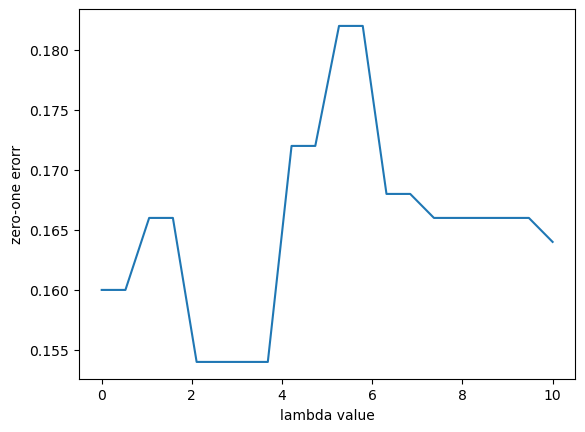
\includegraphics[width=10cm]{homework/homework_3/immages/question_11_1.png}
        \item 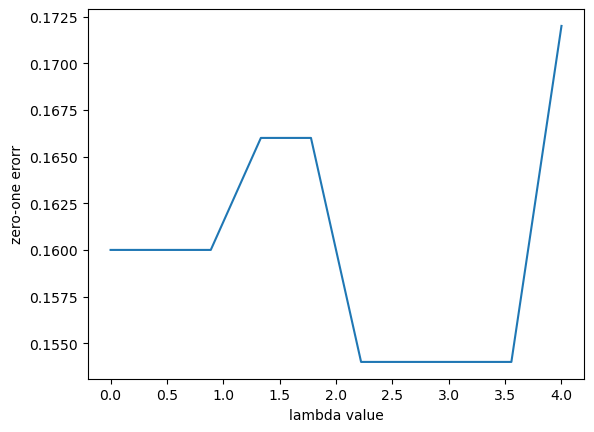
\includegraphics[width=10cm]{homework/homework_3/immages/question_11_2.png}
            \item 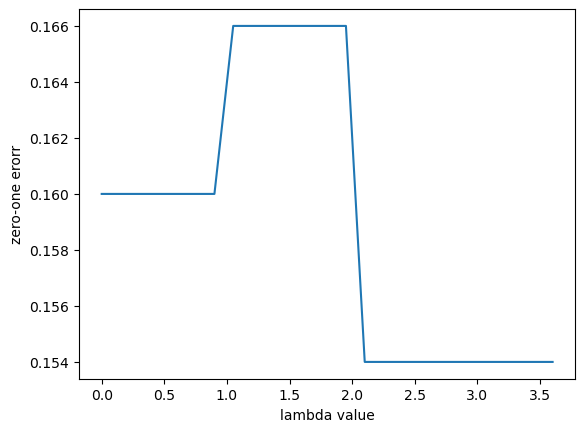
\includegraphics[width=10cm]{homework/homework_3/immages/question_11_3.png}

                \item so i chose my ideal $\lambda$ to be 2
\end{itemize}

\setcounter{saveenum}{\value{enumi}}
\end{enumerate}

\nyuparagrah{\bf Error Analysis {(Optional)}}

Recall that the \emph{score} is the value of the prediction
$f(\bs x)=\bs w^{T} \bs x$. We like to think that the magnitude of the score represents
the confidence of the prediction. This is something we can directly
verify or refute.

\begin{enumerate}
  \setcounter{enumi}{\value{saveenum}}
\item  \textcolor{violet}{(Optional)} Break the predictions on the test set into groups based on the score
(you can play with the size of the groups to get a result you think
is informative). For each group, examine the percentage error. You
can make a table or graph. Summarize the results. Is there a correlation
between higher magnitude scores and accuracy?\\
\begin{itemize}
    \color{blue}
                    \item 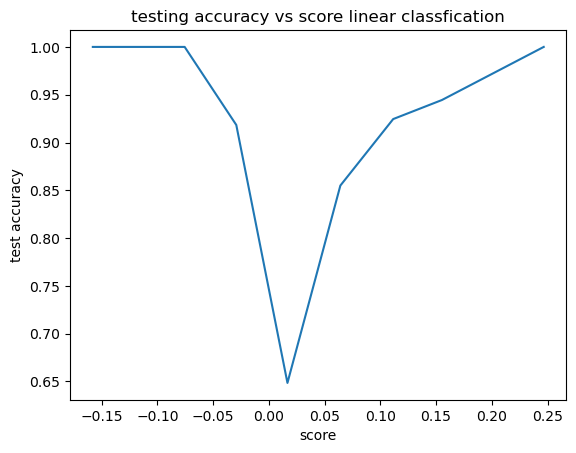
\includegraphics[width=10cm]{homework/homework_3/immages/question_13_1.png}
                    \item 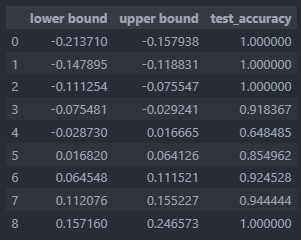
\includegraphics[width=10cm]{homework/homework_3/immages/question_13_2.png.jpg}
    \item yes there was a co relation of absolute value 0.79 of magnitude scores and accuracy
\end{itemize}



\setcounter{saveenum}{\value{enumi}}
\end{enumerate}

In natural language processing 
one can often interpret why a model has performed well or poorly on
a specific example. The
first step in this process is to look closely at the errors that the
model makes.

\begin{enumerate}
  \setcounter{enumi}{\value{saveenum}}
\item \textcolor{nyupurple}{(Optional)} Choose an input example $\bs x=\left(x_{1},\ldots,x_{d}\right)\in\mathbb{R}^{d}$
that the model got wrong. We want to investigate what features contributed
to this incorrect prediction. One way to rank the importance of the
features to the decision is to sort them by the size of their contributions
to the score. That is, for each feature we compute $\left|w_{i}x_{i}\right|$,
where $w_{i}$ is the weight of the $i$th feature in the prediction
function, and $x_{i}$ is the value of the $i$th feature in the input
$x$. Create a table of the most important features, sorted by $\left|w_{i}x_{i}\right|$,
including the feature name, the feature value $x_{i}$, the feature
weight $w_{i}$, and the product $w_{i}x_{i}$. Attempt to explain
why the model was incorrect. Can you think of a new feature that might
be able to fix the issue? Include a short analysis for at least 2
incorrect examples.
% and sometimes it is not very difficult to come
% up with ideas for
Can you think of new features that might help fix a problem? (Think of making groups of words.)
\begin{itemize}
\color{blue}
\item 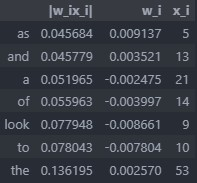
\includegraphics[width=10cm]{homework/homework_3/immages/question_14_1.png.jpg}
\item 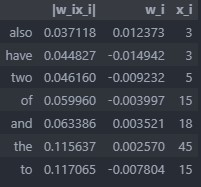
\includegraphics[width=10cm]{homework/homework_3/immages/question_14_2.png.jpg}
\item 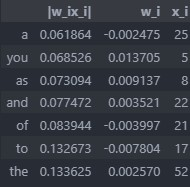
\includegraphics[width=10cm]{homework/homework_3/immages/question_14_3.png.jpg}
    \item for these three examples all the words are very ambiguous. it makes sense that in isolation it is unclear how words like, "as" or "and" should impact classification. Perhaps analyzing these texts with a larger unit of analysis like sentences or groups of words as opposed to single words.
\end{itemize}


\setcounter{saveenum}{\value{enumi}}
\end{enumerate}


\section{\large Kernel Methods}

\subsection{Kernelization review}

Consider the following optimization problem on a data set $\left(\bs x_{1},y_{1}\right),\ldots\left(\bs x_{n},y_{n}\right)\in\mathbb{R}^{d}\times\mathcal{Y}$:
\[
\min_{w\in\mathbb{R}^{d}}R\left(\sqrt{\left\langle \bs w,\bs w\right\rangle }\right)+L\left(\left\langle \bs w,\bs x_{1}\right\rangle ,\ldots,\left\langle \bs w,\bs x_{n}\right\rangle \right),
\]
where $\bs w,\bs x_{1},\ldots,\bs x_{n}\in\mathbb{R}^{d}$, and $\left\langle \cdot,\cdot\right\rangle $
is the standard inner product on $\mathbb{R}^{d}$. The function $R:[0,\infty)\to\mathbb{R}$
is nondecreasing and gives us our regularization term, while $L:\mathbb{R}^{n}\to\mathbb{R}$ is arbitrary\footnote{You may be wondering ``Where are the $y_{i}$'s?''. They're built
into the function $L$. For example, a square loss on a training set
of size $3$ could be represented as $L(s_{1},s_{2},s_{3})=\frac{1}{3}\left[\left(s_{1}-y_{1}\right)^{2}+\left(s_{2}-y_{2}\right)^{2}+\left(s_{3}-y_{3}\right)^{3}\right]$,
where each $s_{i}$ stands for the $i$th prediction $\left\langle \bs w, \bs x_{i}\right\rangle $. } and gives us our loss term. We noted in lecture that this general
form includes soft-margin SVM and ridge regression, though not lasso
regression. Using the representer theorem, we showed if the optimization
problem has a solution, there is always a solution of the form $\bs w=\sum_{i=1}^{n}\bs \alpha_{i} \bs x_{i}$,
for some $\alpha\in\mathbb{R}^{n}$. Plugging this into the our original
problem, we get the following ``kernelized'' optimization problem:
\[
\min_{\bs \alpha\in\mathbb{R}^{n}}R\left(\sqrt{\bs \alpha^{T}K \bs \alpha}\right)+L\left(K\bs \alpha\right),
\]
where $K\in\mathbb{R}^{n\times n}$ is the Gram matrix (or ``kernel matrix'')
defined by $K_{ij}=k(\bs x_{i},\bs x_{j})=\left\langle \bs x_{i}, \bs x_{j}\right\rangle $.
Predictions are given by
\[
f(x)=\sum_{i=1}^{n} \alpha_{i}k(\bs x_{i}, \bs x),
\]
and we can recover the original $\bs w\in\mathbb{R}^{d}$ by $\bs w=\sum_{i=1}^{n}\alpha_{i} \bs x_{i}$.

The \emph{kernel trick} is to swap out occurrences of the
kernel $k$ (and the corresponding Gram matrix $K$) with another
kernel. For example, we could replace $k(x_{i},x_{j})=\left\langle x_{i},x_{j}\right\rangle $
by $k'(x_{i},x_{j})=\left\langle \psi(x_{i}),\psi(x_{j})\right\rangle $
for an arbitrary feature mapping $\bs \psi:\mathbb{R}^{d}\to\mathbb{R}^{d}$.
In this case, the recovered $\bs w\in\mathbb{R}^{d}$ would be $\bs w=\sum_{i=1}^{n}\alpha_{i}\bs \psi(\bs x_{i})$
and predictions would be $\left\langle \bs w, \bs\psi(\bs x_{i})\right\rangle $\@.

More interestingly, we can replace $k$ by another kernel $k''(\bs x_{i}, \bs x_{j})$
for which we do not even know or cannot explicitly write down a corresponding
feature map $\bs \psi$. Our main example of this is the RBF kernel
\[
k(x,x')=\exp\left(-\frac{\|x-x'\|^{2}}{2\sigma^{2}}\right),
\]
for which the corresponding feature map $\psi$ is infinite dimensional.
In this case, we cannot recover $w$ since it would be infinite dimensional.
Predictions must be done using $\alpha\in\mathbb{R}^{n}$, with $f(x)=\sum_{i=1}^{n}\alpha_{i}k(\bs x_{i}, \bs x)$. 

Your implementation of kernelized methods below should not make any
reference to $\bs w$ or to a feature map $\bs \psi$. Your learning
routine should return $\bs \alpha$, rather than $\bs w$, and your prediction
function should also use $\bs \alpha$ rather than $\bs w$. This will allow
us to work with kernels that correspond to infinite-dimensional feature
vectors.

\subsection{Kernel problems}

\nyuparagrah{\bf Ridge Regression: Theory}

Suppose our input space is $\mbox{\ensuremath{\mathcal{X}}=}\mathbb{R}^{d}$ and
our output space is $\mathcal{Y}=\mathbb{R}$. Let $\mathcal{D}=\left\{ \left(\bs x_{1},y_{1}\right),\ldots,\left(\bs x_{n},y_{n}\right)\right\} $
be a training set from $\mathcal{X}\times\mathcal{Y}$. We'll use the ``design matrix''
$X\in\mathbb{R}^{n\times d}$, which has the input vectors as rows: 
\[
X=\begin{pmatrix}-\bs x_{1}-\\
\vdots\\
-\bs x_{n}-
\end{pmatrix}.
\]
Recall the ridge regression objective function:
\[
J(\bs w)=||X\bs w-y||^{2}+\lambda||\bs w||^{2},
\]
for $\lambda>0$.
\begin{enumerate}
  \setcounter{enumi}{\value{saveenum}}
\item Show that for $\bs w$ to be a minimizer of $J(\bs w)$, we must have $X^{T}X\bs w+\lambda I\bs w=X^{T}y$.
Show that the minimizer of $J(\bs w)$ is $\bs w=(X^{T}X+\lambda I)^{-1}X^{T}y$.
Justify that the matrix $X^{T}X+\lambda I$ is invertible, for $\lambda>0$.
(You should use properties of positive (semi)definite matrices. If you need a reminder look up the Appendix.) \\
\begin{itemize}
    \color{blue}
    \item $J(W)=||Xw-y||_{2}^2+\lambda||w||_{2}^2=(w^wx^tXw-w^tX^ty-y^txw)^2+(\lambda w^tW)^2$
    \item we can take the gradient of this to see that $\nabla_{j}(w)=4X^TXw-4X^Ty+4\lambda w$ item setting this equal to zero and solving yields $w^{*}=(X^TX+\lambda I)^{-1}(X^ty)$ as the only extrema of our function so if there is a min it will be at that point 
    \item taking the second derivative yields $4\lambda\geq 0$ so the function is convex,and thus we know $J(W)$ will have one unique minimum at $w^{*}=(X^TX+\lambda I)^{-1}(X^ty)$ 
    \item next we want to show $(X^TX+\lambda I)$ is invertable 
    \begin{itemize}
        \item to show a  matrix is invertable we just need to show it has no zero eigenvalues 
        \item a matrix A is positive definite if $\forall v\in \mathbb{R}^{d} $ $v^tAv>0$
        \item so for an arbitrary vector v we can write $v^t(X^TX+\lambda I)v=v^{t}X^TXv+v^T\lambda I V$
        \item we can see that $v^T(X^TX)v=v^t\Sigma_{i=1}^{d}(x_i)^{t}X_iv=\Sigma_{j=1}^{d}v_j\Sigma_{i=1}^{n}(X^{t}_{i,j}X_{i,j})v_j=\Sigma_{i=1}^{d}\Sigma_{j=1}^{d}(X_{i,j})^2(V_i)^2\geq 0$ since it is the sum of squared quantities 
        \item $v^T\lambda I v=\lambda v^TIv=\lambda v^tv=\lambda ||v||$ for any nonzero vector $v$ $||v||>0$ and $\lambda>0$ thus $v^t\lambda Iv>0 $
        \item so for an arbitrary vector v we can write $v^t(X^TX+\lambda I)v=v^{t}X^TXv+v^T\lambda I v>0$
        \item meaning $v^t(X^TX+\lambda I)v$ is positive definite and thus has no zero eigenvalues 
        \item meaning that $v^t(X^TX+\lambda I)v$ is invertable 
    \end{itemize}
\end{itemize}


\item Rewrite $X^{T}Xw+\lambda Iw=X^{T}y$ as $\bs w=\frac{1}{\lambda}(X^{T}y-X^{T}Xw)$.
Based on this, show that we can write $w=X^{T}\bs \alpha$ for some $\bs \alpha$,
and give an expression for $\bs \alpha$.\\

\begin{itemize}
    \color{blue}
    \item $X^TXw+\lambda Iw=X^ty\Rightarrow \lambda Iw=X^ty-X^TXw\Rightarrow Iw=\frac{1}{\lambda}(X^ty-X^TXw)\\\Rightarrow w=\frac{1}{\lambda}(X^ty-X^TXw)$
    \item we can write $ w=\frac{1}{\lambda}(X^ty-X^TXw)$ as $\frac{1}{\lambda}(X^ty-X^TXw)=X^t\frac{1}{\lambda }(y-Xw)$ and then define $\frac{1}{\lambda }(y-Xw)=\alpha\in \mathbb{R}^{n}$ thus we have $ w=X^{T}\alpha$ which was what we waned to show
\end{itemize}

\item Based on the fact that $\bs w=X^{T}\bs \alpha$, explain why we say $\bs w$ is ``in
the span of the data.''\\
\begin{itemize}
\color{blue}
    \item for a matrix $v\in \mathbb{R}^{n \times d}$ the span of v is def fined as $span(v)=span(v_1...v_n)=\{v_1\alpha_1+v_2\alpha_2+...v_n\alpha_n|\forall \alpha_{i}\in \mathbb{R}\}=\{\Sigma_{i=1}^{n}v_i\alpha_i|\forall \alpha_{i}\in \mathbb{R}\}=\{X^t\alpha|\forall \alpha\in \mathbb{R}^{n}\}$ that is all linear combinations of its rows. 
    \item as we know $X$ is our data matrix and $w=X^{T}\alpha$ it must be the case that $w\in span(X)=span(x_1...x_n)$ that is we can get $w$ as a linear combination of the rows of our data matrix which represent out data points.  
\end{itemize}

\item Show that $\bs \alpha=(\lambda I+XX^{T})^{-1}y$. Note that $XX^{T}$
is the kernel matrix for the standard vector dot product. (Hint: Replace
$\bs w$ by $X^{T}\bs \alpha$ in the expression for $\bs \alpha$, and then solve
for $\bs \alpha$.)\\
\begin{itemize}
    \color{blue}
    \item from question 16 we have $\alpha=\frac{1}{\lambda}y-\frac{1}{\lambda }Xw$ adn given $w=X^T\alpha$ we  can write $\alpha=\frac{1}{\lambda}y-\frac{1}{\lambda }X^t\alpha\Rightarrow\frac{1}{\lambda}y=(I+\frac{1}{\lambda}XX^t)\alpha\Rightarrow\\\frac{1}{\lambda}y(I+\frac{1}{\lambda}XX^t)^{-1}=\alpha\Rightarrow y(\lambda I+XX^t)^{-1}=\alpha$ 
\end{itemize}


\item Give a kernelized expression for the $X\bs w$, the predicted values on
the training points. (Hint: Replace $\bs w$ by $X^{T}\bs \alpha$ and $\bs \alpha$
by its expression in terms of the kernel matrix $XX^{T}$.)\\

\begin{itemize}
\color{blue}
    \item we can write our prediction as $Xw=X(X^T\alpha)=(XX^T)\alpha=\\ 
    \begin{pmatrix}
        <x_1,x_1>&...&<x_1,x_n>\\
        ...&...&...\\
        <x_n,x_1>&...&<x_n,x_n>
    \end{pmatrix}\alpha=K \alpha$ 
\end{itemize}

\item Give an expression for the prediction $f(x)=x^{T}\bs w^{*}$ for a new
point $x$, not in the training set. The expression should only involve
$x$ via inner products with other $\bs x$'s. (Hint: It is often convenient
to define the column vector
\[
k_{\bs x}=\begin{pmatrix}\bs x^{T}\bs x_{1}\\
\vdots\\
\bs x^{T}\bs x_{n}
\end{pmatrix}
\]
to simplify the expression.) \\
\setcounter{saveenum}{\value{enumi}}
\end{enumerate}

\begin{itemize}
   \color{blue}
    \item $\hat{f}(x)=w^tx=<w^*.x>=<\Sigma_{i=1}^{n}\alpha_i^*x_i,x>=\Sigma_{i=1}^{n}<\alpha_i^* x_i,x>=\Sigma_{i=1}^{n}\alpha_i^*< x_i,x>=k_{x}^{t}\alpha^{*}$
\end{itemize}


\nyuparagrah{\bf Kernels and Kernel Machines}

There are many different families of kernels. So far we spoken
about linear kernels, RBF/Gaussian kernels, and polynomial kernels.
The last two kernel types have parameters. In this section, we'll
implement these kernels in a way that will be convenient for implementing
our kernelized ridge regression later on. For simplicity,
%  and because it
% is by far the most common situation, 
we will assume that our input space is $\mathcal{X}=\mathbb{R}$
% ^{d}$\footnote{We are noting this because one interesting aspect of kernel methods
% is that they can act directly on an arbitrary input space $\mathcal{X}$ (e.g.
% text files, music files, etc.), so long as you can define a kernel
% function $k:\mathcal{X}\times\mathcal{X}\to\mathbb{R}.$ But we'll not consider that case
% here.}
.
 This allows
us to represent a collection of $n$ inputs in a matrix $X\in\mathbb{R}^{n\times 1}$. 
You should now refer to the jupyter notebook \texttt{skeleton\_code\_kernels.ipynb}.

\begin{enumerate}
  \setcounter{enumi}{\value{saveenum}}
\item Write functions that compute the RBF kernel $k_{\text{RBF}(\sigma)}(x,x')=\exp\left(-\|x-x'\|^{2}/\left(2\sigma^{2}\right)\right)$
and the polynomial kernel $k_{\text{poly}(a,d)}(x,x')=\left(a+\left\langle x,x'\right\rangle \right)^{d}$.
The linear kernel $k_{\text{linear}}(x,x')=\left\langle x,x'\right\rangle $,
has been done for you in the support code. Your functions should take
as input two matrices $W\in\mathbb{R}^{n_{1}\times d}$ and $X\in\mathbb{R}^{n_{2}\times d}$
and should return a matrix $M\in\mathbb{R}^{n_{1}\times n_{2}}$ where
$M_{ij}=k(W_{i\cdot},X_{j\cdot})$. In words, the $(i,j)$'th entry
of $M$ should be kernel evaluation between $w_{i}$ (the $i$th row
of $W$) and $x_{j}$ (the $j$th row of $X$).
% The matrix $M$ could
% be called the ``cross-kernel'' matrix, by analogy to the \href{https://en.wikipedia.org/wiki/Cross-covariance}{cross-covariance matrix}.
For the RBF kernel, you may use the scipy function \texttt{cdist(X1,X2,'sqeuclidean')}
in the package \texttt{scipy.spatial.distance}. 
% or (with some more
% work) write it in terms of the linear kernel (\href{https://multimedia-pattern-recognition.info/fileadmin/Websites/mmprec/uploads/docs/Bauckhage/np-sp-rec-edm.pdf}{Bauckhage's article}
% on calculating Euclidean distance matrices may be helpful).
\begin{itemize}
    \color{blue}
      \inputminted[firstline=1110, lastline=1136, breaklines=True]{python}{hw_3.py}
\end{itemize}


\item Use the linear kernel function defined in the code to compute the
kernel matrix on the set of points $x_{0}\in\mathcal{D}_{X}=\left\{ -4,-1,0,2\right\} $.
Include both the code and the output. 

\begin{itemize}

      \inputminted[firstline=433, lastline=434, breaklines=True]{python}{hw_3.py}

    \color{blue}
    \item here is the output 
    \item 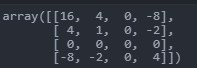
\includegraphics[width=10cm]{homework/homework_3/immages/question_22_1.png.jpg}
\end{itemize}
\item Suppose we have the data set $\mathcal{D}_{X,y}= \left\{ (-4,2),(-1,0),(0,3),(2,5)\right\} $ (in each set of parentheses, the first number is the value of $x_i$ and the second number the corresponding value of the target $y_i$).
Then by the representer theorem, the final prediction function will
be in the span of the functions $x\mapsto k(x_{0},x)$ for $x_{0}\in\mathcal{D}_{X}=\left\{ -4,-1,0,2\right\} $.
This set of functions will look quite different depending on the kernel
function we use. The set of functions $x\mapsto k_{\text{linear}}(x_{0},x)$ for
$x_{0}\in\mathcal{X}$ and for $x\in[-6,6]$ has been provided for the linear kernel.
\begin{enumerate}
  % \setcounter{enumi}{\value{saveenum}}
\item Plot the set of functions $x\mapsto k_{\text{poly(1,3)}}(x_{0},x)$
for $x_{0}\in\mathcal{D}_{X}$ and for $x\in[-6,6]$.
\item Plot the set of functions $x\mapsto k_{\text{RBF(1)}}(x_{0},x)$ for
$x_{0}\in\mathcal{X}$ and for $x\in[-6,6]$.
% \setcounter{saveenum}{\value{enumi}}
\end{enumerate}
Note that the values of the parameters of the kernels you should use are given in their definitions in (a) and (b).
\begin{itemize}
    \color{blue}
    \item 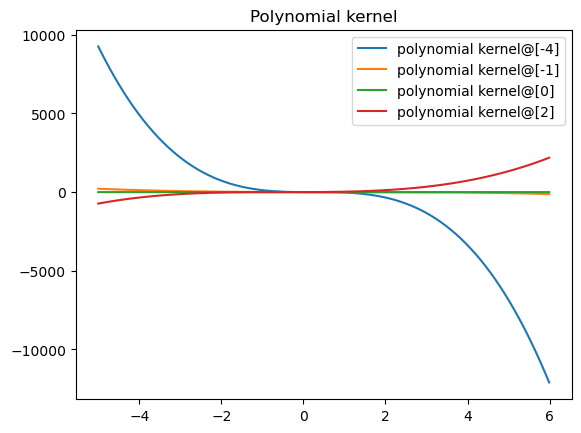
\includegraphics[width=10cm]{homework/homework_3/immages/question_23_1.png}
        \item 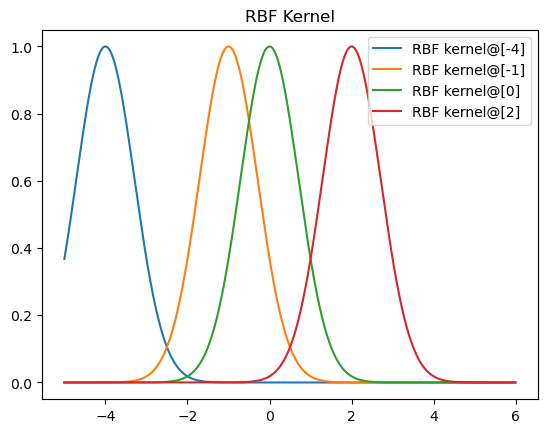
\includegraphics[width=10cm]{homework/homework_3/immages/question_23_2.png}
\end{itemize}

\item By the representer theorem, the final prediction function will be
of the form $f(x)=\sum_{i=1}^{n}\alpha_{i}k(x_{i},x)$, where $x_{1},\ldots,x_{n}\in\mathcal{X}$
are the inputs in the training set. 
% This is a special case of what
% is sometimes called a \textbf{\href{https://davidrosenberg.github.io/ml2015/docs/4c.kernels.pdf\#page=16}{kernel machine}},
% which is a function of the form $f(x)=\sum_{i=1}^{r}\alpha_{i}k(\mu_{i},x)$,
% where $\mu_{1},\ldots,\mu_{r}\in\mathcal{X}$ are called \textbf{prototypes}
% or \textbf{centroids} (Murphy's book Section 14.3.1.). In the special
% case that the kernel is an RBF kernel, we get what's called an \textbf{RBF
% Network} (proposed by \href{http://sci2s.ugr.es/keel/pdf/algorithm/articulo/1988-Broomhead-CS.pdf}{Broomhead and Lowe in 1988}).
We will use the class \texttt{Kernel\_Machine} in the skeleton code to make prediction with different kernels.
% We can see that the prediction functions we get from our kernel methods
% will be kernel machines in which each input in the training set $x_{1},\ldots,x_{n}$
% serves as a prototype point. 
Complete the \texttt{predict} function
of the class \texttt{Kernel\_Machine}. Construct
a \texttt{Kernel\_Machine} object with the RBF kernel (sigma=1), with
prototype points at $-1,0,1$ and corresponding weights $\alpha_i$ $1,-1,1$.
Plot the resulting function.\\
\begin{itemize}
    \color{blue}
    
    \item here is the plot of
    \item 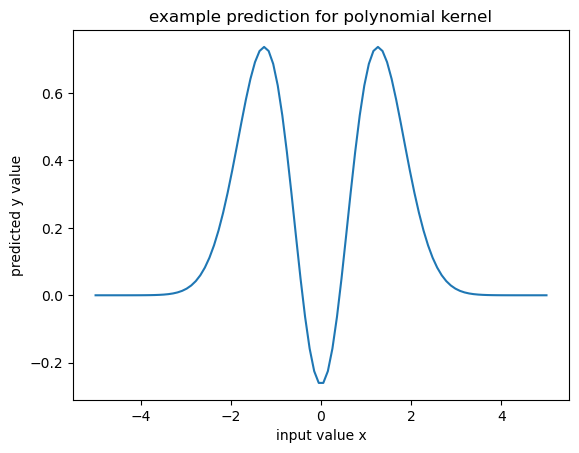
\includegraphics[width=10cm]{homework/homework_3/immages/question_24_1.png}
\end{itemize}

\setcounter{saveenum}{\value{enumi}}
\end{enumerate}

Note: For this last problem, and for other problems below, it may be helpful
to use \href{https://en.wikipedia.org/wiki/Partial_application}{partial application}
on your kernel functions. For example, if your polynomial kernel function
has signature \texttt{polynomial\_kernel(W, X, offset, degree)}, you
can write \texttt{k = functools. partial(polynomial\_kernel, offset=2,
degree=2)}, and then a call to \texttt{k(W,X)} is equivalent to \texttt{polynomial\_kernel(W,
X, offset=2, degree=2)}, the advantage being that the extra parameter
settings are built into \texttt{k(W,X)}. This can be convenient so
that you can have a function that just takes a kernel function \texttt{k(W,X)}
and doesn't have to worry about the parameter settings for the kernel.

\nyuparagrah{\bf Kernel Ridge Regression: Practice}

In the zip file for this assignment, we provide a training \texttt{krr-train.txt} and test
set \texttt{krr-test.txt} for a one-dimensional
regression problem, in which $\mathcal{X}=\mathcal{Y}=\mathcal{A}=\mathbb{R}$. Fitting this
data using kernelized ridge regression, we will compare the results
using several different kernel functions. Because the input space
is one-dimensional, we can easily visualize the results.

\begin{enumerate}
  \setcounter{enumi}{\value{saveenum}}
\item Plot the training data. You should note that while there is a clear
relationship between $x$ and $y$, the relationship is not linear.
\begin{itemize}
    \color{blue}
    \item 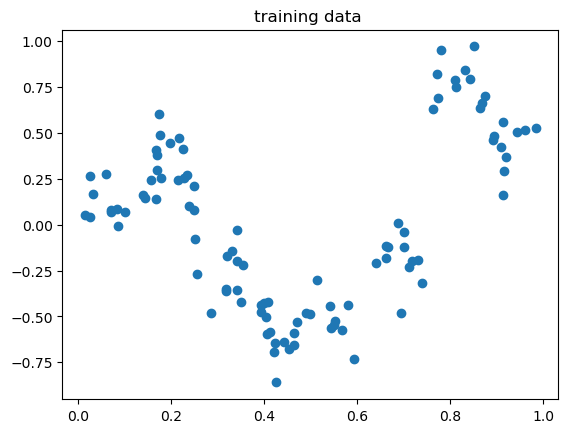
\includegraphics[width=10cm]{homework/homework_3/immages/question_25_1.png}
\end{itemize}

\item In a previous problem, we showed that in kernelized ridge regression,
the final prediction function is $f(\bs x)=\sum_{i=1}^{n}\alpha_{i}k(\bs x_{i},\bs x)$,
where $\alpha=(\lambda I+K)^{-1}y$ and $K\in\mathbb{R}^{n\times n}$
is the kernel matrix of the training data: $K_{ij}=k(\bs x_{i},\bs x_{j})$,
for $\bs x_{1},\ldots, \bs x_{n}$. In terms of kernel machines, $\alpha_{i}$
is the weight on the kernel function evaluated at the training point
$\bs x_{i}$. Complete the function \texttt{train\_kernel\_ridge\_regression}
so that it performs kernel ridge regression and returns a \texttt{Kernel\_Machine}
object that can be used for predicting on new points. 
\begin{itemize}
    \color{blue}
      \inputminted[firstline=481, lastline=505, breaklines=True]{python}{hw_3.py}
\end{itemize}



\item Use the code provided to plot your fits to the training data for the
RBF kernel with a fixed regularization parameter of $0.0001$ for
3 different values of sigma: $0.01$, $0.1$, and $1.0$. What values
of sigma do you think would be more likely to over fit, and which
less? \\

\begin{itemize}
    \color{blue}
    \item 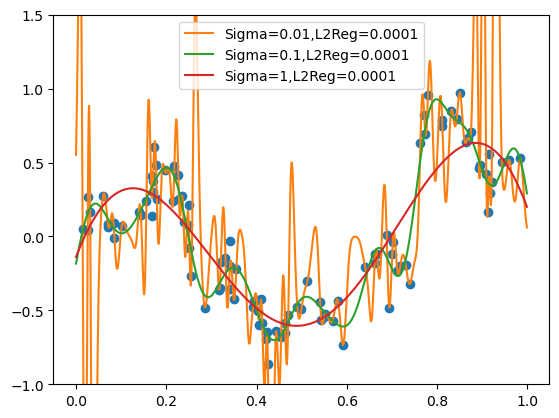
\includegraphics[width=10cm]{homework/homework_3/immages/question_27_1.png}
    \item it seems that low values of sigma are very sensitive to changes in the training data so they are more likely to over-fit than lower values of sigma
\end{itemize}

\item Use the code provided to plot your fits to the training data for the
RBF kernel with a fixed sigma of $0.02$ and 4 different values of
the regularization parameter $\lambda$: $0.0001$, $0.01$, $0.1$,
and $2.0$. What happens to the prediction function as $\lambda\to\infty$?
\begin{itemize}
    \color{blue}
    \item 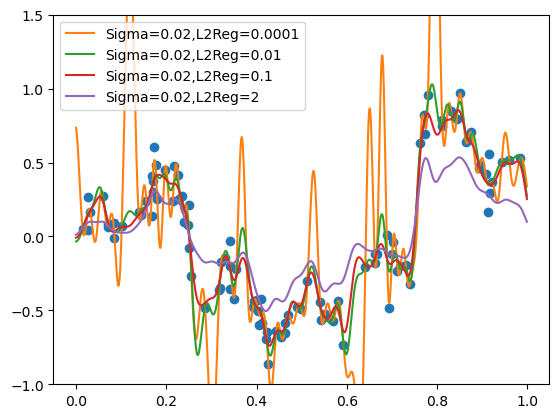
\includegraphics[width=10cm]{homework/homework_3/immages/question_28_1.png}
    \item it seems that low values of $\lambda$ are very sensitive to changes in the training data so they are more likely to over-fit while it looks like very high values of $\lambda$ lead to under fitting to the training data 
\end{itemize}

\item \textcolor{violet}{(Optional)} Find the best hyperparameter settings (including kernel parameters
and the regularization parameter) for each of the kernel types. Summarize
your results in a table, which gives training error and test error
for each setting. Include in your table the best settings for each
kernel type, as well as nearby settings that show that making small
change in any one of the hyperparameters in either direction will
cause the performance to get worse. You should use average square
loss on the test set to rank the parameter settings. To make things
easier for you, we have provided an sklearn wrapper for the kernel
ridge regression function we have created so that you can use sklearn's
GridSearchCV. Note: Because of the small dataset size, these models
can be fit extremely fast, so there is no excuse for not doing extensive
hyperparameter tuning. 
\begin{itemize}
    \color{blue}
    \item 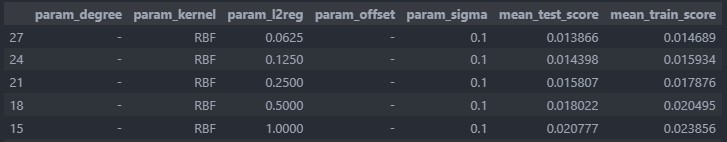
\includegraphics[width=10cm]{homework/homework_3/immages/question_29_1.png}
    \item 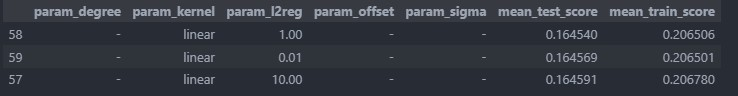
\includegraphics[width=10cm]{homework/homework_3/immages/question_29_2.png}
    \item 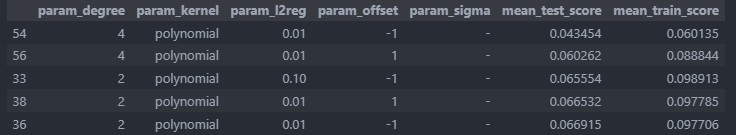
\includegraphics[width=10cm]{homework/homework_3/immages/question_29_3.png}
\end{itemize}

\item \textcolor{violet}{(Optional)} Plot your best fitting prediction functions using the polynomial kernel
and the RBF kernel. Use the domain $x\in\left(-0.5,1.5\right)$. Comment
on the results. 
\begin{itemize}
    \color{blue}
    \item 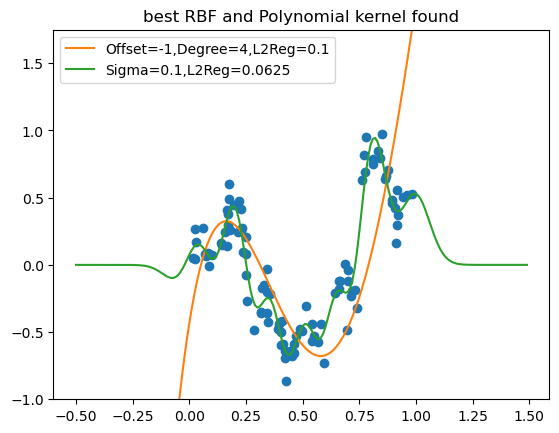
\includegraphics[width=10cm]{homework/homework_3/immages/question_30_1.png}
    \item both kernel ls seem to capture the data really well. 
    \item it is possible that the polynomial kernel is better as it is fitting the general shape with out getting thrown off by points that might be noise

\end{itemize}


\item \textcolor{violet}{(Optional)} The data for this problem was generated as follows: A function $f:\mathbb{R}\to\mathbb{R}$
was chosen. Then to generate a point $\left(x,y\right)$, we sampled
$x$ uniformly from $(0,1)$ and we sampled $\eps\sim\mathcal{N}\left(0,0.1^{2}\right)$
(so $var(\eps)=0.1^{2}$). The final point is $\left(x,f(x)+\eps\right)$.
What is the Bayes decision function and the Bayes risk for the loss
function $\ell\left(\hat{y},y\right)=\left(\hat{y}-y\right)^{2}$.\\
\begin{itemize}
    \color{blue}
    \item the Bayes function is defined as $f^{*}:\mathcal{X}\Rightarrow \mathcal{A}: f^{*}\in argmin_{f}R(F)$ 
    \item in this context the risk of a function g can be expressed as \\$R(g)=E_{(x,f(x)+\epsilon)\sim P(x\times y)[\ell(g(x),y)]=E_{(x,f(x)+\epsilon)\sim P(x\times y)[(g(x)-f(x)+\epsilon)^2]$
    \item $\epsilon$ is a random quantity so we can not really minimize the risk around it, thus our Bayes function will be $f^{*}(x)=f(x)$
    \item thus we can calculate our Bayes risk as \\$R(f^*)=E_{(x,f(x)+\epsilon)\sim P(x\times y)}[(f^*(x)-f(x)+\epsilon)^2]=E_{(x,f(x)+\epsilon)\sim P(x\times y)}[(f(x)-f(x)+\epsilon)^2]=E_{(x,f(x)+\epsilon)\sim P(x\times y)}[(\epsilon)^2]=var(\epsilon)=.1^2$
    \item this makes sense as even if we fully capture the deterministic function we are trying to understand $\epsilon$ is still present as an irreducible level of noise
\end{itemize}



\setcounter{saveenum}{\value{enumi}}
\end{enumerate}


\section{Kernel SVMs with Kernelized
Pegasos (Optional)}

\begin{enumerate}
  \setcounter{enumi}{\value{saveenum}}
\item \textcolor{violet}{(Optional)} Load the SVM training \texttt{svm-train.txt} and \texttt{svm-test.txt} test data from the zip file.
Plot the training data using the code supplied. Are the data linearly
separable? Quadratically separable? What if we used some RBF kernel?

\begin{itemize}
     \color{blue}
     \item the data looks like there is a Circe of one class so rounding the other class
    \item No the data is not linearly seperable
    \item since they are thus ceperated by what looks aproxently like a circle it is likely that either an rbh or quadratic kernel should be able to seperate the data.
\end{itemize}

\item \textcolor{violet}{(Optional)} Unlike for kernel ridge regression, there is no closed-form
    solution for SVM classification (kernelized or not). Implement kernelized
Pegasos. Because we are not using a sparse representation for this
data, you will probably not see much gain by implementing the ``optimized''
versions described in the problems above.
\begin{itemize}
    \color{blue}
      \inputminted[firstline=1124, lastline=1209, breaklines=True]{python}{hw_3.py}
\end{itemize}


\item \textcolor{violet}{(Optional)} Find the best hyperparameter settings (including kernel
parameters and the regularization parameter) for each of the kernel
types. Summarize your results in a table, which gives training error
and test error (i.e. average $0/1$ loss) for each setting. Include
in your table the best settings for each kernel type, as well as nearby
settings that show that making small change in any one of the hyperparameters
in either direction will cause the performance to get worse. You should
use the $0/1$ loss on the test set to rank the parameter settings. 
\begin{itemize}
    \color{blue}
    \item 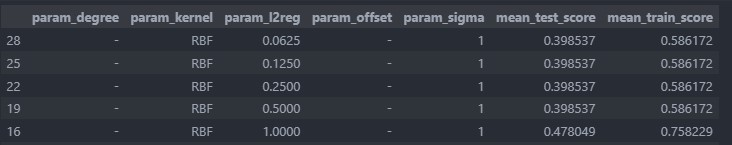
\includegraphics[width=10cm]{homework/homework_3/immages/question_34_1.png}
    \item 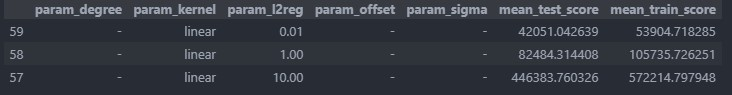
\includegraphics[width=10cm]{homework/homework_3/immages/question_34_2.png}
    \item 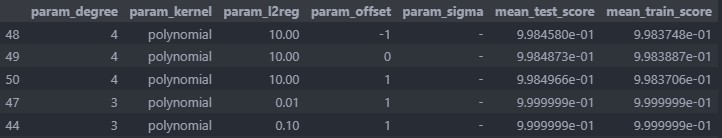
\includegraphics[width=10cm]{homework/homework_3/immages/question_34_3.png}
\end{itemize}


\item \textcolor{violet}{(Optional)} Plot your best fitting prediction functions using the
linear, polynomial, and the RBF kernel. The code provided may help.
\begin{itemize}
    \color{blue}
    \item 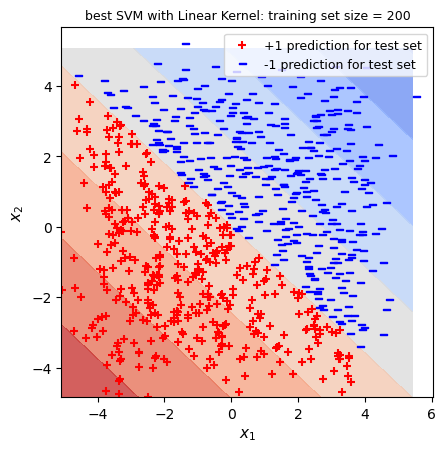
\includegraphics[width=10cm]{homework/homework_3/immages/question_35_1.png}
    \item 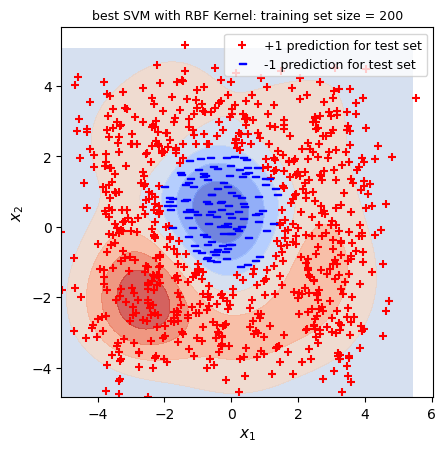
\includegraphics[width=10cm]{homework/homework_3/immages/question_35_2.png}
    \item 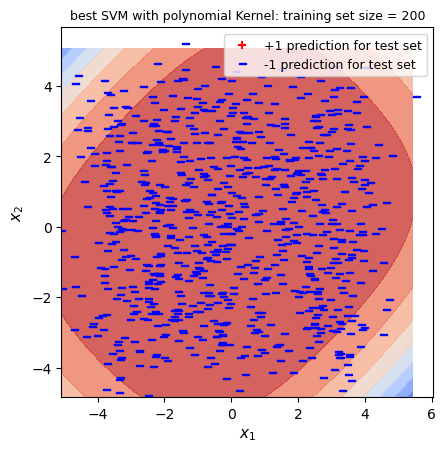
\includegraphics[width=10cm]{homework/homework_3/immages/question_35_3.png}
\end{itemize}



\setcounter{saveenum}{\value{enumi}}
\end{enumerate}

\newpage

\appendix
{ \huge \bf Appendix (Not for credit)} \\[.2cm]

Here we are recalling important properties of positive (semi)definite matrices. 
The exercises below are for revisions for student who may not feel comfortable with these notions.  \textbf{None of the appendix is for credit. }

\section{Positive Semidefinite Matrices}

In statistics and machine learning, we use positive semidefinite matrices
a lot. Let's recall some definitions from linear algebra that will
be useful here:

{\bf Definition. }
A set of vectors $\left\{ x_{1},\ldots,x_{n}\right\} $ is \textbf{orthonormal}
if $\left\langle x_{i},x_{i}\right\rangle =1$ for any $i\in\left\{ 1,\ldots,n\right\} $
(i.e. $x_{i}$ has unit norm), and for any $i,j\in\left\{ 1,\ldots,n\right\} $
with $i\neq j$ we have $\left\langle x_{i},x_{j}\right\rangle =0$
(i.e. $x_{i}$ and $x_{j}$ are orthogonal).

Note that if the vectors are column vectors in a Euclidean space,
we can write this as $x_{i}^{T}x_{j}=\ind{i\neq j}$ for all $i,j\in\left\{ 1,\ldots,n\right\} $. 
%\end{defn*}

{\bf Definition. }
A matrix is \textbf{orthogonal }if it is a square matrix with orthonormal
columns. 

It follows from the definition that if a matrix $M\in\mathbb{R}^{n\times n}$
is orthogonal, then $M^{T}M=I$, where $I$ is the $n\times n$ identity
matrix. Thus $M^{T}=M^{-1}$, and so $MM^{T}=I$ as well. 
%\end{defn*}

{\bf Definition. }
A matrix $M$ is \textbf{symmetric }if $M=M^{T}$. 
%\end{defn*}

{\bf Definition. }
For a square matrix $M$, if $Mv=\lambda v$ for some column vector
$v$ and scalar $\lambda$, then $v$ is called an \textbf{eigenvector}
of $M$ and $\lambda$ is the corresponding \textbf{eigenvalue}. 
%\end{defn*}

{\bf Theorem. }
[Spectral Theorem]A real, symmetric matrix $M\in\mathbb{R}^{n\times n}$
can be diagonalized as $M=Q\Sigma Q^{T}$, where $Q\in\mathbb{R}^{n\times n}$
is an orthogonal matrix whose columns are a set of orthonormal eigenvectors
of $M$, and $\Sigma$ is a diagonal matrix of the corresponding eigenvalues. 
% \end{thm*}

{\bf Definition. }
A real, symmetric matrix $M\in\mathbb{R}^{n\times n}$ is \textbf{positive
semidefinite (psd)} if for any $x\in\mathbb{R}^{n}$, 
\[
x^{T}Mx\ge0.
\]

Note that unless otherwise specified, when a matrix is described as
positive semidefinite, we are implicitly assuming it is real and symmetric
(or complex and Hermitian in certain contexts, though not here).

As an exercise in matrix multiplication, note that for any matrix
$A$ with columns $a_{1},\ldots,a_{d}$, that is 
\[
A=\begin{pmatrix}| &  & |\\
a_{1} & \cdots & a_{d}\\
| &  & |
\end{pmatrix}\in\mathbb{R}^{n\times d},
\]
we have
\[
A^{T}MA=\begin{pmatrix}a_{1}^{T}Ma_{1} & a_{1}^{T}Ma_{2} & \cdots & a_{1}^{T}Ma_{d}\\
a_{2}^{T}Ma_{1} & a_{2}^{T}Ma_{2} & \cdots & a_{2}^{T}Ma_{d}\\
\vdots & \vdots & \cdots & \vdots\\
a_{d}^{T}Ma_{1} & a_{d}^{T}Ma_{2} & \cdots & a_{d}^{T}Ma_{d}
\end{pmatrix}.
\]
So $M$ is psd if and only if for any $A\in\mathbb{R}^{n\times d}$, we
have $diag(A^{T}MA)=\left(a_{1}^{T}Ma_{1},\ldots,a_{d}^{T}Ma_{d}\right)^{T}\succeq0$,
where $\succeq$ is elementwise inequality, and $0$ is a $d\times1$
column vector of $0$'s . 
%\end{defn*}
\begin{enumerate}
\item Use the definition of a psd matrix and the spectral theorem to show
that all eigenvalues of a positive semidefinite matrix $M$ are non-negative.
{[}Hint: By Spectral theorem, $\Sigma=Q^{T}MQ$ for some $Q$. What
if you take $A=Q$ in the ``exercise in matrix multiplication''
described above?{]} \textbf{}\\
\item In this problem, we show that a psd matrix is a matrix version of
a non-negative scalar, in that they both have a ``square root''.
Show that a symmetric matrix $M$ can be expressed as $M=BB^{T}$
for some matrix $B$, if and only if $M$ is psd. {[}Hint: To show
$M=BB^{T}$ implies $M$ is psd, use the fact that for any vector
$v$, $v^{T}v\ge0$. To show that $M$ psd implies $M=BB^{T}$ for
some $B$, use the Spectral Theorem.{]}\\
\end{enumerate}

\section{Positive Definite Matrices}
{\bf Definition. }
A real, symmetric matrix $M\in\mathbb{R}^{n\times n}$ is \textbf{positive
definite} (spd) if for any $x\in\mathbb{R}^{n}$ with $x\neq0$, 
\[
x^{T}Mx>0.
\]
%\end{defn*}
\begin{enumerate}
\item Show that all eigenvalues of a symmetric positive definite matrix
are positive. {[}Hint: You can use the same method as you used for
psd matrices above.{]} 
\item Let $M$ be a symmetric positive definite matrix. By the spectral
theorem, $M=Q\Sigma Q^{T}$, where $\Sigma$ is a diagonal matrix
of the eigenvalues of $M$. By the previous problem, all diagonal
entries of $\Sigma$ are positive. If $\Sigma=diag\left(\sigma_{1},\ldots,\sigma_{n}\right)$,
then $\Sigma^{-1}=diag\left(\sigma_{1}^{-1},\ldots,\sigma_{n}^{-1}\right)$.
Show that the matrix $Q\Sigma^{-1}Q^{T}$ is the inverse of $M$. 
\item Since positive semidefinite matrices may have eigenvalues that are
zero, we see by the previous problem that not all psd matrices are
invertible. Show that if $M$ is a psd matrix and $I$ is the identity
matrix, then $M+\lambda I$ is symmetric positive definite for any
$\lambda>0$, and give an expression for the inverse of $M+\lambda I$.
\item Let $M$ and $N$ be symmetric matrices, with $M$ positive semidefinite
and $N$ positive definite. Use the definitions of psd and spd to
show that $M+N$ is symmetric positive definite. Thus $M+N$ is invertible.
(Hint: For any $x\neq0$, show that $x^{T}(M+N)x>0$. Also note that
$x^{T}(M+N)x=x^{T}Mx+x^{T}Nx$.) 
\end{enumerate}


\end{document}